\setcounter{chapter}{2}
\chapter{Kết quả}
\section{Mô tả dữ liệu}
Dữ liệu nhóm thu thập được bao gồm 4 file csv sau:
\begin{itemize}
	\item File CustomberBase.csv chứa thông tin của 5674 khác hàng với các thuộc tính như Cust\_ID - mã số của khách hàng, Age - là tuổi của khách hàng, Customer\_Segment - hạng của khách hàng, Customer\_Vintage\_Group - nhóm khách hàng thuộc vào.
	\item File CardBase.csv chứa thông tin của 500 thẻ tương ứng với 500 chủ sở hữu trong 5674 người thuộc file CustomberBase.csv. File này chứa các thuộc tính Card\_Number - số thẻ, Card\_Family - loại thẻ, Credit\_Limit - số tiền giới hạn của thẻ, Cust\_ID - mã số của chủ thẻ.
	\item File TransactionBase.csv chứa thông tin của các giao dịch trong năm 2016 tương ứng với thẻ trong file CardBase.csv. File này chứa các thuộc tính Transaction\_ID - mã số giao dịch, Transaction\_Date - thời gian giao dịch, Credit\_Card\_ID - số thẻ tham gia giao dịch, Transaction\_Value - số lượng tiền giao dịch, Transaction\_Segment - phân lớp giao dịch.
\end{itemize}
\textit{Chú ý:} Lý do bảo mật nên mọi thông tin về số thẻ, khách hàng, lượng tiền giao dịch đều đã bị thay đổi.

Ta biến đổi dữ liệu trên thành các file csv, mỗi file chứa thông tin giao dịch của chủ thẻ trong năm 2016, được chia thành hai phần: dữ liệu giao dịch đầu tiên tới giao dịch áp chót dùng trong việc luyện mô hình, giao dịch cuối cùng cho việc kiểm tra mô hình. Tổng số dữ liệu kiểm tra là 470 giao dịch trong đó gồm: 67 giao dịch có nhãn gian lận và 403 giao dịch chính thống.

Dữ liệu giao dịch của mỗi người rất ít, mỗi thẻ chỉ có 6 - 20 giao dịch cho việc luyện mô hình. Đây là hạn chế lớn của dữ liệu, ảnh hưởng không tốt tới kết quả của mô hình.

Từ những dữ liệu nhóm đã có sẵn, với mỗi chủ thẻ, ta xây dựng mô hình Markov ẩn với số lượng lớp ẩn là 4, số lượng kí hiệu quan sát là 3, các ma trận $A,\; B,\; \pi$ đều được khởi tạo với phân phối đều.

\section{Kết quả}
Các tiêu chuẩn để đánh giá mô hình:
\begin{itemize}
	\item Accuracy - tỷ lệ số lượng dự đoán đúng so với số lượng dữ liệu kiểm tra.
	\item Confusion matrix 
	
	$$
	\begin{bmatrix} 
		TN & FP \\
		FN & TP \\
	\end{bmatrix}
	$$

	TP (True positive) - số lượng giao dịch gian lận được dự đoán chính xác.
	
	FP (False positive) - số lượng giao dịch chính thống nhưng bị dự đoán là gian lận.
	
	TN (True negative) - số lượng giao dịch chính thống được dự đoán chính xác.
	
	FP (False Negative) - số lượng giao dịch gian lận nhưng bị dự đoán là chính thống.
	\item Precision: $$\frac{TP}{TP+FP}$$
	\item Recall:
	$$\frac{TP}{TP+FN}$$
\end{itemize}

Với ngưỡng là $0.4$ ta thu được các kết quả đánh giá sau:
\begin{itemize}
	\item Accuracy$=0.9$.
	\item Precision$=0.622$.
	\item Recall$=0.7612$.
	\item Confusion matrix:
	
	$$
	\begin{bmatrix} 
	372 & 31 \\
	16 & 51 \\
	\end{bmatrix}
	$$
	
\end{itemize}

Với bộ dữ liệu còn thiếu hụt thì mô hình trên ổn nhưng chưa đủ để ứng dụng vào thực tế.

Khảo sát sự thay đổi của ngưỡng ảnh hưởng tới kết quả của mô hình:
\begin{center}
	
	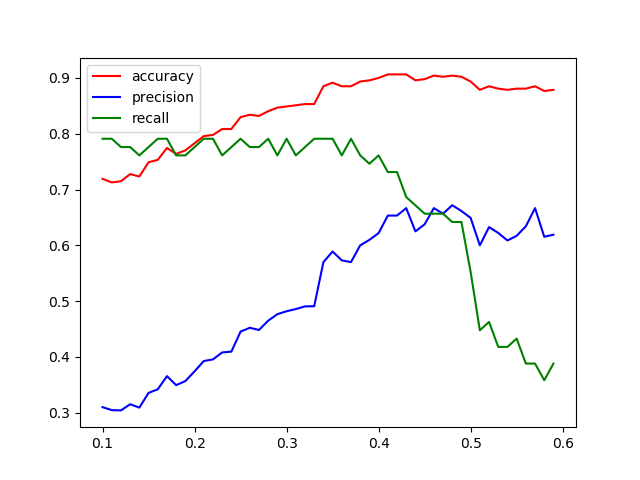
\includegraphics[scale=1]{31.png}
	
	
	\textit{Hình 3.1:} Đồ thị thể hiện sự ảnh hưởng của ngưỡng.
\end{center}
Từ hình trên ta thấy việc chọn ngưỡng rất quan trọng. Nếu ngưỡng quá cao hệ thống sẽ bỏ qua nhiều gian lận trong khi nếu ngưỡng quá thấp thì hệ sẽ báo nhiều giao dịch chính thống là gian lận.